\begin{appendices}
	
	\chapter{Summary}
	All organisms have a genome made of DNA (deoxyribonucleic acid).
	The genome can be found in nearly every cell and is the blueprint for the growth, development, maintenance and repair of the body.
	It performs these functions by transcribing small pieces of DNA, the genes, from the genome and translating them to proteins.
	These proteins are the tiny workhorses of the body that break down food, give bones their strength, make muscles move, let brains think, and so on.
	There are many thousands of different genes and proteins with each their own task.
	
	The genome is copied from cell to cell, and is inherited from generation to generation.
	The copying process is incredibly precise, but always makes a few little mistakes.
	These so-called mutations cause small differences between individuals, so that natural selection and thus evolution can take place.
	Unfortunately, mutations can also cause detrimental effects, such as genetic disorders.
	When the function of a gene is disrupted by a mutation, a specific disorder can arise.
	For a lot of genes it is known which disorder they can cause, but for most genes we do not know what happens when they are disrupted.
	
	In this thesis we research and develop various bioinformatics models, methods en systems to elucidate which genes and DNA differences can make people ill.
	To support the research into genes, we develop a database in chapter \ref{chap:xgap}.
	This database is useful for collecting all kinds of biological data.
	Chapter \ref{chap:xqtl} presents software to analyze these data as an extension to this database.
	This software can determine which region of the genome is responsible for diseases and other physical traits.
	
	Organisms such as rat, worm or zebrafish allow us to perform research that would be impractical or unethical on humans.
	These studies deliver valuable biological insights, but it is often remains unclear how those insights can help us to understand human disorders.
	In Chapter \ref{chap:wormqtl} we report the development of an interactive database that connects research into worms to the genetics of human disease.
	Despite the fact that worms do not look much like humans, they have thousands of genes that work exactly the same way as in humans.
	By looking at disorders, physical traits and genes in both organisms we discover new ways to use worms for research into human diseases.
	
	Next to understanding the genes lies the challenge to determine the harmfulness (pathogenicity) of new mutations.
	Each individual carries many unique mutations no one else has.
	This makes it challenging to find the causal mutation for a patient with a genetic disorder.
	We can use our knowledge of the genome and evolution to predict how pathogenic new mutations are.
	In chapter \ref{chap:caddmmr} we report a smart new method which predict which mutations are harmless and which cause hereditary colon cancer.
	This works rather well and we make recommendations for the guideline that establishes diagnoses.
	
	Encouraged by these results we expanded our scope from just a few to thousands of disease genes in chapter \ref{chap:gavin}.
	For this, we use DNA from individuals that have no connection to severe disorders.
	We compared that to disease causing mutations that were found in patients.
	By crunching the numbers for every gene, it is determined when a mutation is probably disease causing.
	The final result is a public website where the DNA of patients can be scanned quickly and accurately for probable pathogenic mutations.
	
	Finally, chapter \ref{chap:frameworkforgenomics} describes how we developed a system for automated DNA analysis, including a protocol specific for genome diagnostics.
	This protocol uses our new method but also the latest knowledge on mutations and genes.
	Pathogenic mutations are not always responsible for the disease of a patient.
	That is why the DNA of family members is used to determine if the genetic pieces of the patient truly fit.
	The output is a new file format in which medically relevant information is formally expressed.
	This file can be converted to a clear report in which the most important information is found at the top.
	
	One of the advantages is that we can apply this analysis without manual work to the genomes of thousands of healthy people.
	The results act as a control that tells us how often the software returns an accidental hit in each gene.
	By stating this information in the final report, medical experts can focus their attention on genes with the fewest accidental hits.
	This increases the speed and confidence at which a genetic diagnosis is established for the patient.
	
	\chapter{Samenvatting}
	Alle organismen hebben een genoom dat is opgebouwd uit DNA (desoxyribonucleïnezuur).
	Het genoom zit in bijna elke cel en is de blauwdruk voor de groei, ontwikkeling, onderhoud en herstel van het lichaam.
	Het vervult deze functies door kleine stukjes DNA, de genen, van het genoom af te schrijven en deze te vertalen naar eiwitten.
	Deze eiwitten zijn de werkpaardjes van het lichaam die voedsel afbreken, botten hun sterkte geven, spieren laten bewegen, hersenen laten denken, enzovoort.
	Er zijn vele duizenden verschillende genen en eiwitten met allemaal hun eigen taak.
	
	Het genoom wordt gekopieerd van cel naar cel, en wordt overgeërfd van generatie op generatie.
	Het kopieerproces is ongelofelijk precies, maar maakt altijd wel een paar foutjes.
	Deze zogeheten mutaties zorgen voor kleine verschillen tussen individuen, waardoor natuurlijke selectie en dus evolutie kan plaatsvinden.
	Helaas kunnen mutaties ook nadelige effecten veroorzaken, zoals erfelijke ziektes.
	Wanneer de werking van een gen verstoord wordt door een mutatie kan een bepaalde ziekte optreden.
	Van een hoop genen is bekend welke ziekte ze kunnen veroorzaken, maar van de meeste genen weten we niet wat er gebeurt wanneer ze verstoord worden.
	
	In dit proefschrift onderzoeken en ontwikkelen we verscheidene bioinformatica modellen, methoden en systemen om op te helderen welke genen en DNA verschillen mensen ziek kunnen maken.
	Om het onderzoek naar genen te ondersteunen, ontwikkelen we een database in hoofdstuk \ref{chap:xgap}.
	Deze database is handig voor het verzamelen van allerlei biologische gegevens.
	Als uitbreiding op deze database presenteert hoofdstuk \ref{chap:xqtl} software voor de analyse van deze gegevens.
	Deze software kan bepalen welk gebied van het genoom verantwoordelijk is voor ziektes en andere uiterlijke kenmerken.
	
	Dieren zoals rat, worm en zebravis stellen ons in staat om onderzoek te doen die onpraktisch of onethisch zou zijn op mensen.
	Deze onderzoeken leveren waardevolle biologische inzichten op, maar het blijft vaak onduidelijk hoe die inzichten ons kunnen helpen om ziektes in de mens te begrijpen.
	In hoofdstuk \ref{chap:wormqtl} rapporteren we de ontwikkeling van een interactieve database die het onderzoek naar wormen verbindt aan de genetica van menselijke ziektes.
	Ondanks het feit dat wormen niet echt op mensen lijken, hebben zij duizenden genen die precies hetzelfde werken als bij mensen.
	Door te kijken naar ziektes, uiterlijke kenmerken en genen in beide organismen ontdekken we nieuwe manieren om wormen te gebruiken voor onderzoek naar menselijke ziektes.
	
	Naast het begrijpen van de genen ligt de uitdaging om de schadelijkheid (pathogeniciteit) van nieuwe mutaties te bepalen.
	Ieder individu draagt vele unieke mutaties die niemand anders heeft.
	Dit maakt het een uitdaging om de schuldige mutatie te vinden bij een patient met een genetische ziekte.
	We kunnen onze kennis van het genoom en de evolutie inzetten om te voorspellen hoe pathogeen nieuwe mutaties zijn.
	In hoofdstuk \ref{chap:caddmmr} rapporteren we een slimme nieuwe methode die voorspelt welke mutaties ongevaarlijk zijn en welke erfelijke darmkanker veroorzaken.
	Dit blijkt vrij goed te kunnen en we doen aanbevelingen voor de richtlijn die diagnoses stelt.
	
	Aangemoedigd door deze resultaten zijn we onze speelruimte gaan uitbreiden van slechts een paar tot wel duizenden ziektegenen in hoofdstuk \ref{chap:gavin}.
	Hiervoor gebruiken we DNA van mensen die geen verband hebben met ernstige ziektes.
	Dat vergelijken we met ziekteverwekkende mutaties die bij patienten gevonden zijn.
	Met het nodige rekenwerk voor ieder gen wordt bepaald wanneer een mutatie waarschijnlijk ziekteverwekkend is.
	Het resultaat is een openbare website waar het DNA van patienten snel en accuraat gescand kan worden op mogelijk pathogene mutaties.
	
	Tenslotte beschrijft hoofdstuk \ref{chap:frameworkforgenomics} hoe we een systeem voor geautomatiseerde DNA analyse ontwikkeld hebben, inclusief een protocol specifiek voor genoom diagnostiek.
	Dit protocol gebruikt onze nieuwe methode maar ook de laatste kennis over mutaties en genen.
	Pathogene mutaties zijn niet altijd verantwoordelijk voor de ziekte van een patient.
	Daarom wordt het DNA van familieleden gebruikt om te bepalen of het genetische plaatje bij de patient ook echt klopt.
	De uitvoer is een nieuw bestandsformaat waarin medisch relevante informatie formeel wordt uitgedrukt.
	Dit bestand kan worden omgezet naar een overzichtelijk rapport waarin de meest belangrijke informatie bovenaan staat.
	
	Eén van de voordelen is dat we deze analyse zonder handwerk kunnen toepassen op de genomen van duizenden gezonde mensen.
	De uitkomst hiervan dient als controle die ons verteld hoe vaak de software een toevalstreffer heeft in elk gen.
	Door deze informatie in het uiteindelijke rapport te vermelden kunnen medisch experts hun aandacht richten op genen met de minste toevalstreffers.
	Hiermee wordt de snelheid en zekerheid waarmee een genetische diagnose bij de patient wordt vastgesteld, verhoogd.
	
	\chapter{Acknowledgements}
	
	\newpage
	~\\~\\~\\~\\~\\
	
	\chapter{Dankwoord}
	Het schrijven van dit dankwoord is misschien het moeilijkste deel van dit proefschrift, want in de jaren dat ik hier op de afdeling genetica werk hebben zoveel mensen mij bijgestaan, zowel voor als tijdens mijn promotietraject. Het is daarom onmogelijk om iedereen die dank verdient bij naam te noemen. Enkele mensen wil ik toch bij naam noemen.\\
	
	\noindent Allereerst, Dr. Raddatz, beste Birgit, reeds in 2001, tijdens mijn stage op de afdeling genetica was jij mijn begeleider. Samen met Gineke en de rest van de FISH-groep heb je me geïntroduceerd in de genetische diagnostiek. Na een korte uitstap bij de prenatale cytogenetische diagnostiek, kwam ik in 2005 weer bij jou in de groep te werken. Ook na de reorganisatie en de oprichting van ‘team 3’ volgde ik jou naar de nieuwe werkzaamheden. In de afgelopen (bijna) 18 jaar heb ik zoveel van je geleerd en je stond (en staat) altijd klaar voor een vraag of steuntje in de rug wanneer ik het nodig heb, of om me naar huis te sturen wanneer ik te lang doorwerk. Ik ben daarom ook blij dat je mijn co-promotor bent.\\ 
	
	\noindent Prof. Dr. Sijmons, beste Rolf, onze wegen hebben elkaar voor het eerst gekruist bij de heroprichting van de Genehoppers waar we ons met de belangrijkste activiteit van de afdeling genetica bezig hielden: muziek maken. Bij de oprichting van de sectie ontwikkeling en innovatie in 2012 waarin ‘team 3’ werd opgenomen, kwam ik bij jou werken. Ik zal nooit vergeten dat ik enkele jaren later vertelde dat ik na het afronden van mijn master wijsbegeerte (dat nog een aantal jaren in de toekomst lag) graag een PhD traject in zou willen gaan. Je reactie was: “goed idee, maar we gaan niet wachten tot je de master hebt afgerond”. Het gevolg is dat ik hier nu zit, nog steeds zonder master in de wijsbegeerte, maar met proefschrift. Hartelijk dank voor alle kansen die je me hebt geboden, de vrijheid die je me hebt gegeven en je onaflatende enthousiasme.\\ 
	
	\noindent Prof. Dr. Swertz, beste Morris, ik wil ook jou hartelijk bedanken voor de kansen die je me hebt geboden en de begeleiding in de afgelopen jaren. In 2012 gaf je me de gelegenheid om een stage te lopen binnen de GCC en mede daaruit zijn de onderwerpen ontstaan die uiteindelijk de basis vormen van dit proefschrift. Ik ben ook erg blij dat ik na mijn promotie als postdoc in jouw team aan de slag kan.\\ 
	
	\noindent I would like to express my gratitude to Prof. Dr. V.V.A.M Knoers, Prof. Dr. J.K. Ploos van Amstel and Prof. Dr. M. Vihinen for making room in your schedules to assess my thesis.\\ 
	
	\noindent Prof. dr. J.W. Romeijn, beste Jan-Willem, hartelijk dank voor het commentaar op de epistemologische reflectie.\\
	
	\noindent Ook wil ik mijn paranimfen bedanken. Ik ben vereerd dat jullie hier vandaag naast mij willen staan. Eddy, ik ken je al sinds ik bij de prenatale cytogenetica kwam werken en de bijdrage die je aan dit proefschrift hebt geleverd is van onschatbare waarde. Elk jaar kijk ik ook uit naar onze reizen. Met jou heb ik de grootste avonturen beleefd op zoek naar de grootste slagvelden van de afgelopen eeuwen. Samen hebben we de slag bij Waterloo overleefd en na ons uitstapje naar Borodino weet ik dat we vanuit elke plaats de weg naar huis terug zullen vinden. Krista, bij de oprichting van ‘team 3’ werden we collega’s. Jij met de DNA expertise en ik vanuit de chromosomenhoek. Ik heb veel van je geleerd over het detecteren en interpreteren van varianten.\\ 
	
	\noindent I would like to thank all the past and current colleagues of the O\&I section for interesting discussions and collaborations.\\ 
	
	\noindent Mohamed, we have worked closely together the past four years. I have enjoyed our discussions and the ‘African viewpoint’. It was a sad moment when you returned to Tanzania, but I look forward to come and visit you in the near future.\\
	
	\noindent Helga, thank you for your work on ‘the onco paper’ and your advice on people/promotor management.\\
	
	\noindent A warm thanks to all past and present GCC colleagues. I remember when the GCC started within the department and I had to share the coffee machine with those strange bio-informaticians. In the past years we have also shared quite a lot of beers and hotpots. Undoubtedly many more will follow. I am happy to get the opportunity to work more closely with you in the coming years.\\
	
	\noindent Freerk, toen mijn stage bij de GCC begon was jij mijn buurman en tot de introductie van de flexplekken zijn we dat gebleven. Bedankt voor de hulp bij al mijn domme vragen en voor de prettige samenwerking bij het ontwikkelen van CoNVaDING. Veel succes bij je nieuwe baan in Utrecht.\\
	
	\noindent Edgar, bedankt voor de gezelligheid. Je aanwezigheid wordt nog elke dag gemist in de ‘stilte’-kamer.\\
	
	\noindent I would like to thank Jackie Senior and Kate Mc Intyre for editing all the chapters that made it into this thesis. I am sorry for the many words I sent for the reflection/discussion.\\ 
	
	\noindent Ook bedankt aan alle stagiaires die ik de afgelopen jaren heb mogen begeleiden. Ik heb wellicht meer geleerd van jullie dan jullie van mij. Dirk, bedankt voor je onmisbare bijdrage aan het NIPT project.\\
	
	\noindent Huidige en oud-collega’s van de genoomdiagnostiek, bedankt voor de goede samenwerking en de begeleiding in mijn jonge jaren. De jaren aan ADL4 zal ik nooit vergeten.\\
	
	\noindent Dr. E.L.M. Maeckelberghe, beste Els, en alle deelnemers aan de maandelijkse ethiekbijeenkomsten, heel erg bedankt voor de discussies over de meest uiteenlopende onderwerpen.  Jullie hebben mijn perspectief aanzienlijk verbreed.\\
	
	\noindent Mama en papa, bedankt dat jullie mij een geweldige jeugd hebben gegeven en dat jullie nog altijd voor mij klaar staan. Een bezoek aan jullie is altijd een rustpunt in het drukke leven. Papa, helaas is er geen diner met Carl XVI Gustaf gepland, dat bleek toch bij een ander feestje te horen.\\
	
	\noindent Carien, Johan, Gerhard, Rianne en Leonie, bedankt dat de deur bij jullie altijd open staat. Bij jullie is het altijd gezellig.\\
	
	\noindent Lieve Kim, ik ben elke dag blij dat je er bent. Het leven is zoveel leuker met jou en de jongens. Bedankt voor het aanhoren van al mijn verzuchtingen. Alexander en Thomas, bedankt voor alle leuke dingen die ik met jullie mag doen en dat jullie mij leren dat er meer in het leven is dan werken (zoals trampoline springen). 
	
	\chapter{About the author}
	
	\begin{wrapfigure}{r}{0.33\textwidth}
		\begin{center}
			\includegraphics[width=0.33\textwidth]{img/Lennart_Johansson}
		\end{center}
	\end{wrapfigure}
	Leonard Fredericus (Lennart) Johansson was born in Uithuizen, The Netherlands, on May 29th 1980. 
	After completion of the VWO at Het Hogeland College in Warffum in 1998 he followed the biology and medical laboratory research track of the bachelor Life Sciences and Technology at the Hanze University Groningen and obtained a BASc in 2002, graduating on the implementation of comparative genomic hybridization for the purpose of hematological malignancies at the University Medical Center Groningen (UMCG) department of genetics. 
	In 2015 he obtained a BA in philosophy at the University of Groningen. 
	In his thesis he formulated an answer to the question: ‘does new knowledge about existing results give a moral duty to recontact in clinical genetics?’. 
	He has been working at the UMCG department of genetics since 2002, starting in genome diagnostics and later switching to the development and innovation section where he started his PhD in 2015 under the guidance of Rolf Sijmons, Birgit Raddatz and Morris Swertz, of which the results are presented in this thesis.
	
	\chapter{List of publications}
	
	\section{Published}*
	\begin{enumerate}
		\item Targeted next-generation sequencing can replace Sanger sequencing in clinical diagnostics. Sikkema-Raddatz B, \textbf{Johansson LF}, de Boer EN, Almomani R, Boven LG, van den Berg MP, Spaendonck-Zwarts KY, van Tintelen JP, Sijmons RH, Jongbloed JDH, Sinke RJ. \textsl{Human Mutation}. 2013;34(7):1035-42.
	\item Successful noninvasive trisomy 18 detection using single molecule sequencing. van den Oever JME, Balkassmi S, \textbf{Johansson LF}, Adama van Scheltema PN, Suijkerbuijk RF, Hoffer MJV, Sinke RJ, Bakker E, Sikkema-Raddatz B,  Boon EMJ. \textsl{Clinical Chemistry}. 2013;59(1):705-9.
	\item Next-generation sequencing-based genome diagnostics across clinical genetics centers: implementation choices and their effects. Vrijenhoek T, Kraaijeveld K, Elferink M, de Ligt J,  Kranendonk E, Santen G, Nijman IJ, Butler D, Claes G, Costessi A, Dorlijn W, van Eyndhoven W, Halley DJJ, van den Hout MCGN, van Hove S, \textbf{Johansson LF}, Jongbloed JDH, Kamps R, Kockx CEM, de Koning B, Kriek M, Lekanne dit Deprez R, Lunstroo H, Mannens M, Mook OR, Nelen M, Ploem C, Rijnen M, Saris JJ, Sinke R, Sistermans E, van Slegtenhorst M, Sleutels F, van der Stoep N, van Tienhoven M, Vermaat M, Vogel M, Waisfisz Q, Weiss JM, van den Wijngaard A, van Workum W, Ijntema H, van der Zwaag B, Van Ijcken WFJ, den Dunnen J, Veltman JA, Hennekam R, Cuppen E. \textsl{European Journal of Human Genetics}. 2015;23(9);1142-50.
	\item Whole-exome sequencing is a powerful approach for establishing the etiological diagnosis in patients with intellectual disability and microcephaly. Rump P, Jazayeri O, van Dijk-Bos KK, \textbf{Johansson LF}, van Essen AJ, Verheij JBGM, Veenstra-Knol HE, Redeker EJW, Mannens MMAM, Swertz MA, Alizadeh BZ, van Ravenswaaij-Arts CMA, Sinke RJ, Sikkema-Raddatz B. \textsl{BMC medical genomics}. 2016;9(1):7
	\item CoNVaDING: single exon variation detection in targeted NGS data. \textbf{Johansson LF}*, van Dijk F*, de Boer EN, van Dijk-Bos KK, Jongbloed JDH, van der Hout AH, Westers H, Sinke RJ, Swertz MA, Sijmons RH, Sikkema-Raddatz B. \textsl{Human Mutation}. 2016;37(5):457-64.
	\item NIPTRIC: an online tool for clinical interpretation of non-invasive prenatal testing (NIPT) results. Sikkema-Raddatz B, \textbf{Johansson LF}, de Boer EN, Boon EMJ, Suijkerbuijk RF, Bouman K, Bilardo CM, Swertz MA, Dijkstra M, van Langen IM, Sinke RJ, te Meerman GJ. \textsl{Scientific reports}. 2016;6:38659.
	\item Novel algorithms for improved sensitivity in non-invasive prenatal testing. \textbf{Johansson LF}*, de Boer EN*, de Weerd HA, van Dijk F, Elferink MG, Schuring-Blom GH, Suijkerbuijk RF, Sinke RJ, te Meerman GJ, Sijmons GJ, Swertz MA, Sikkema-Raddatz B. \textsl{Scientific reports}.2017;7;1838.
	\item Genetic Screening Test to Detect Translocations in Acute Leukemias by Use of Targeted Locus Amplification. Alimohamed MZ*, \textbf{Johansson LF}*, de Boer EN, Splinter E, Klous P, Yilmaz M, Bosga A, van Min M, Mulder AB, Vellenga E, Sinke RJ, Sijmons RH, van den Berg E, Sikkema-Raddatz B. \textsl{Clinical Chemistry}. 2018;64(7):1096-1103.
	\item NIPTeR: an R package for fast and accurate trisomy prediction in non-invasive prenatal testing. \textbf{Johansson LF}, de Weerd HA, de Boer EN, van Dijk F, te Meerman GJ, Sijmons RH, Sikkema-Raddatz B, Swertz MA. \textsl{BMC bioinformatics}. 2018;19(1):531.
	\end{enumerate}
	
	\section{Accepted}*
	\begin{enumerate}
		\item A next-generation sequencing method for gene doping detection that distinguishes low levels of plasmid DNA against a background of genomic DNA. de Boer EN, Ettema P, \textbf{Johansson LF}, van Diemen CC, Haisma HJ. \textsl{Gene Therapy}.
	\end{enumerate}
	
	\section{Submitted}*
	\begin{enumerate}
		\item What if we would use a diagnostic multi-cancer gene panel for opportunistic screening? A study in 2,090 Dutch familial cancer patients.  \textbf{Johansson LF}, van Dijk-Bos KK, van der Hout AH, Knopperts AP, Leegte B, van den Akker PC, Kok K, van Langen IM , Swertz MA, Weersma RK, Sinke RJ, Sikkema-Raddatz B, Westers H*,  Sijmons RH*.
		\item Reinterpretation, reclassification, and its downstream effects: Challenges for clinical laboratory geneticists. el Mecky J*; \textbf{Johansson L}*; Plantinga M; Fenwick A; Lucassen A; Dijkhuizen T; van der Hout A; Lyle K; van Langen I.
		\item Variant re-interpretation in next-generation sequencing data increases diagnostic yield in 2002 Dutch cardiomyopathy patients. Alimohamed MZ, \textbf{Johansson LF}, Posafalvi A, Boven LG, van Dijk KK, Walters L, Vos YJ, Westers H, Hoedemaekers YM, Sinke RJ, Sijmons RH, Sikkema-Raddatz B, Jongbloed JDH*, van der Zwaag PA*
		\item VIBE: a pipeline-friendly software tool for genome diagnostics to prioritize genes by matching patient symptoms to literature. van der Velde KJ*, van den Hoek S*, van Dijk F, van Diemen CC, \textbf{Johansson LF}, Abbott KM, Deelen P, Sikkema-Raddatz B, Swertz MA. 
		\item Unresolved severe hypercholesterolemia in a cohort of Emiratis with high prevalence of type 2 diabetes mellitus. Rimbert A, Kuivenhoven JA, Buckley A, Lansberg P, Viel M, Kanninga R, \textbf{Johansson L}; Dullaart RPF, Sinke RJ, al Tikriti A, Daggag H, Taysir Barakat M.
	\end{enumerate}
	
	\section{Dutch}*
	\begin{enumerate}
		\item Next-generation sequencing nader bekeken. de Boer EN, \textbf{Johansson LF}. Analyse september 2014;69(4):125-9 \\
	\end{enumerate}
	
	* Shared first or last author
	
	\chapter{Other academic activities}
	
	\begin{table}
		\footnotesize
		\begin{tabulary}{\linewidth}{LL}
			Date & Activity \\
			\hline
			\rule{0pt}{2.5ex}\mbox{01-09-2012} & Participated in the GSMS Project Management course \\
			\rule{0pt}{2.5ex}\mbox{06-09-2012} & Attended the 20th Annual GBB Symposium \\
			\rule{0pt}{2.5ex}\mbox{12-09-2012} & Attended the BioSHaRE Annual Meeting, Paris \\
			\rule{0pt}{2.5ex}\mbox{27-09-2012} & Gave an oral presentation at the LFN Symposium, Wageningen \\
			\rule{0pt}{2.5ex}\mbox{08-11-2012} & Participated in the PhD Introduction Event, Ezinge \\
			\rule{0pt}{2.5ex}\mbox{19-11-2012} & Attended the Connecting Biobanks Meeting, Utrecht \\
			\rule{0pt}{2.5ex}\mbox{28-11-2012} & Participated in the course 'Introduction to HL7/DCM' \\
			\rule{0pt}{2.5ex}\mbox{03-12-2012} & Participated in the Nordic BBMRI Meeting, Tartu \\
			\rule{0pt}{2.5ex}\mbox{07-01-2013} & Talked at the ENCODE Journal Club about machine learning\\
			\rule{0pt}{2.5ex}\mbox{13-03-2013} & Visited dermatology clinic at Instytut Matki i Dziecka, Warsaw \\
			\rule{0pt}{2.5ex}\mbox{19-03-2013} & Attended the CTMM TraIT Symposium, Utrecht \\
			\rule{0pt}{2.5ex}\mbox{03-04-2013} & Gave an oral presentation at the TarGet Conference \\
			\rule{0pt}{2.5ex}\mbox{16-04-2013} & Presented a poster at the NBIC Conference, Lunteren \\
			\rule{0pt}{2.5ex}\mbox{16-04-2013} & Reviewed a paper for J. of the Am. Medical Informatics Assoc.  \\
			\rule{0pt}{2.5ex}\mbox{14-05-2013} & Received the BOSC 2013 Student Travel Award \\
			\rule{0pt}{2.5ex}\mbox{17-06-2013} & Participated in the SYSGENET MC Meeting, Prague \\
			\rule{0pt}{2.5ex}\mbox{18-06-2013} & Gave an oral presentation at the BOSC Conference, Berlin \\
			\rule{0pt}{2.5ex}\mbox{25-06-2013} & Visited the dept. of Genetics at the University of Leicester \\
			\rule{0pt}{2.5ex}\mbox{01-07-2013} & Supervised internship student Mark de Haan \\
			\rule{0pt}{2.5ex}\mbox{11-07-2013} & Reviewed a paper for Journal of Web Semantics \\
			\rule{0pt}{2.5ex}\mbox{26-08-2013} & Participated in the GOPHER/RUG PhD Day \\
			\rule{0pt}{2.5ex}\mbox{11-09-2013} & Gave an oral presentation at the BMB Meeting, Dusseldorf \\
			\rule{0pt}{2.5ex}\mbox{12-09-2013} & Presented a poster at the CTMM Annual Meeting, Utrecht \\
			\rule{0pt}{2.5ex}\mbox{04-11-2013} & Gave an oral presentation at the BioShare AM, Barcelona \\
			\rule{0pt}{2.5ex}\mbox{21-11-2013} & Attended the HandsOn Biobanks Conference, The Hague\\
			\rule{0pt}{2.5ex}\mbox{12-12-2013} & Visited several research groups at the EBI, Hinxton \\
			\rule{0pt}{2.5ex}\mbox{01-01-2014} & Supervised graduation student Pieter Dopheide \\
			\rule{0pt}{2.5ex}\mbox{01-01-2014} & Supervised graduation student Mark de Haan \\
			\rule{0pt}{2.5ex}\mbox{28-01-2014} & Talked at ADCB Journal Club about Deng \textsl{et al.} (Science) \\
			\rule{0pt}{2.5ex}\mbox{23-02-2014} & Attended the Joint RD-Connect Meeting, Heidelberg \\
			\rule{0pt}{2.5ex}\mbox{20-05-2014} & Gave an oral presentation at the HVP5 Conference, Paris \\
			\rule{0pt}{2.5ex}\mbox{31-05-2014} & Presented a poster and satellite talk at ESHG Conference, Milan \\
			\rule{0pt}{2.5ex}\mbox{01-07-2014} & Supervised graduation student Tommy de Boer \\
			\rule{0pt}{2.5ex}\mbox{20-08-2014} & Taught a course segment at UMCG Biobanking Summer School \\
			\hline
		\end{tabulary}
		\caption[Other academic activities, pt. 1/2]{Other academic activities, pt. 1/2.}
		\label{table:appendix_activities_1}
	\end{table}
	
	\begin{table}
		\footnotesize
		\begin{tabulary}{\linewidth}{LL}
			Date & Activity \\
			\hline
			\rule{0pt}{2.5ex}\mbox{12-09-2014} & Written a Jan Kornelis de Cock grant proposal \\
			\rule{0pt}{2.5ex}\mbox{20-09-2014} & Participated in the GOPHER/RUG PhD Day \\
			\rule{0pt}{2.5ex}\mbox{28-10-2014} & Taught course segment at VKGL/VKGN NGS diagn., Rotterdam \\
			\rule{0pt}{2.5ex}\mbox{28-11-2014} & Presented a poster at Connecting Biobanks Conference, Leiden \\
			\rule{0pt}{2.5ex}\mbox{01-01-2015} & Supervised internship student Marieke Bijlsma \\
			\rule{0pt}{2.5ex}\mbox{19-01-2015} & Talked at ADCB Journal Club about Leiserson \textsl{et al.} (Nat. Gen.) \\
			\rule{0pt}{2.5ex}\mbox{02-02-2015} & Reviewed a paper submission for ISMB/ECCB \\
			\rule{0pt}{2.5ex}\mbox{31-03-2015} & Participated in the course 'Introd. to Genetic Epidem. Research' \\
			\rule{0pt}{2.5ex}\mbox{06-06-2015} & Presented a poster at the ESHG Conference, Glasgow \\
			\rule{0pt}{2.5ex}\mbox{11-06-2015} & Attended the GSMS PhD Development Conference \\
			\rule{0pt}{2.5ex}\mbox{25-06-2015} & Talked at the Epigenome Journal Club about DIY analysis in R \\
			\rule{0pt}{2.5ex}\mbox{01-07-2015} & Supervised graduation student Marieke Bijlsma \\
			\rule{0pt}{2.5ex}\mbox{10-07-2015} & Presented a poster at the BOSC Conference, Dublin \\
			\rule{0pt}{2.5ex}\mbox{22-09-2015} & Taught course segment at VKGL/VKGN NGS diagn., Rotterdam \\
			\rule{0pt}{2.5ex}\mbox{05-11-2015} & Talked at ADCB Journal Club about Itan \textsl{et al.} (PNAS) \\
			\rule{0pt}{2.5ex}\mbox{01-01-2016} & Supervised graduation student Mariska Slofstra \\
			\rule{0pt}{2.5ex}\mbox{01-01-2016} & Supervised graduation student Thom Steenhuis \\
			\rule{0pt}{2.5ex}\mbox{18-02-2016} & Participated in the ProjectFactory course by TOC consultants \\
			\rule{0pt}{2.5ex}\mbox{04-03-2016} & Written a BBMRI voucher on variant data sharing\\
			\rule{0pt}{2.5ex}\mbox{21-03-2016} & Participated in the course 'Publishing in English gr.c' \\
			\rule{0pt}{2.5ex}\mbox{14-04-2016} & Talked at ADCB Journal Club about Zhu \textsl{et al.} (Nat. Gen.) \\
			\rule{0pt}{2.5ex}\mbox{21-05-2016} & Presented a poster and a satellite talk at ESHG, Barcelona \\
			\rule{0pt}{2.5ex}\mbox{01-06-2016} & Reviewed a paper for The American Journal of Human Genetics \\
			\rule{0pt}{2.5ex}\mbox{03-09-2016} & Gave an oral presentation at the ECCB Conference, The Hague \\
			\rule{0pt}{2.5ex}\mbox{20-09-2016} & Taught course segment at VKGL/VKGN NGS diagn., Rotterdam \\
			\rule{0pt}{2.5ex}\mbox{11-10-2016} & Taught a course segment at MPDI TopMaster course I \\
			\rule{0pt}{2.5ex}\mbox{03-11-2016} & Talked at ADCB Journal Club about Turpin \textsl{et al.} (Nat. Gen.) \\
			\rule{0pt}{2.5ex}\mbox{19-12-2016} & Reviewed a paper for Genome Biology \\
			\rule{0pt}{2.5ex}\mbox{03-07-2017} & Visited the SciLifeLab Clinical Genomics facility, Stockholm \\
			\rule{0pt}{2.5ex}\mbox{07-09-2017} & Started to supervise graduation student Sander van den Hoek\\
			\rule{0pt}{2.5ex}\mbox{11-09-2017} & Taught course segment at VKGL/VKGN NGS diagn., Rotterdam \\
			\rule{0pt}{2.5ex}\mbox{02-10-2017} & Participated in Bioschemas Adoption Meeting at EBI, Hinxton \\
			\rule{0pt}{2.5ex}\mbox{09-10-2017} & Started to supervise internship student Peer Ketelaars\\
			\rule{0pt}{2.5ex}\mbox{16-11-2017} & Gave an oral presentation at the NASPM Conference, Høvik \\
			\hline
		\end{tabulary}
		\caption[Other academic activities, pt. 2/2]{Other academic activities, pt. 2/2.}
		\label{table:appendix_activities_2}
	\end{table}
	
\end{appendices}

\clearpage
\pagestyle{empty}

\noindent
\textbf{Back cover image explained}\\
The back cover shows an altered version of the Arecibo message, send out on 16 November 1974 from the Arecibo Observatory in Puerto Rico. Key numbers were updated, the antenna dish graphic left out, and it was extended for medical genetics / bioinformatics. The original transmission was broadcasted with a power of 1,000 kW towards globular star cluster M13, which it will reach in roughly 25,000 years.

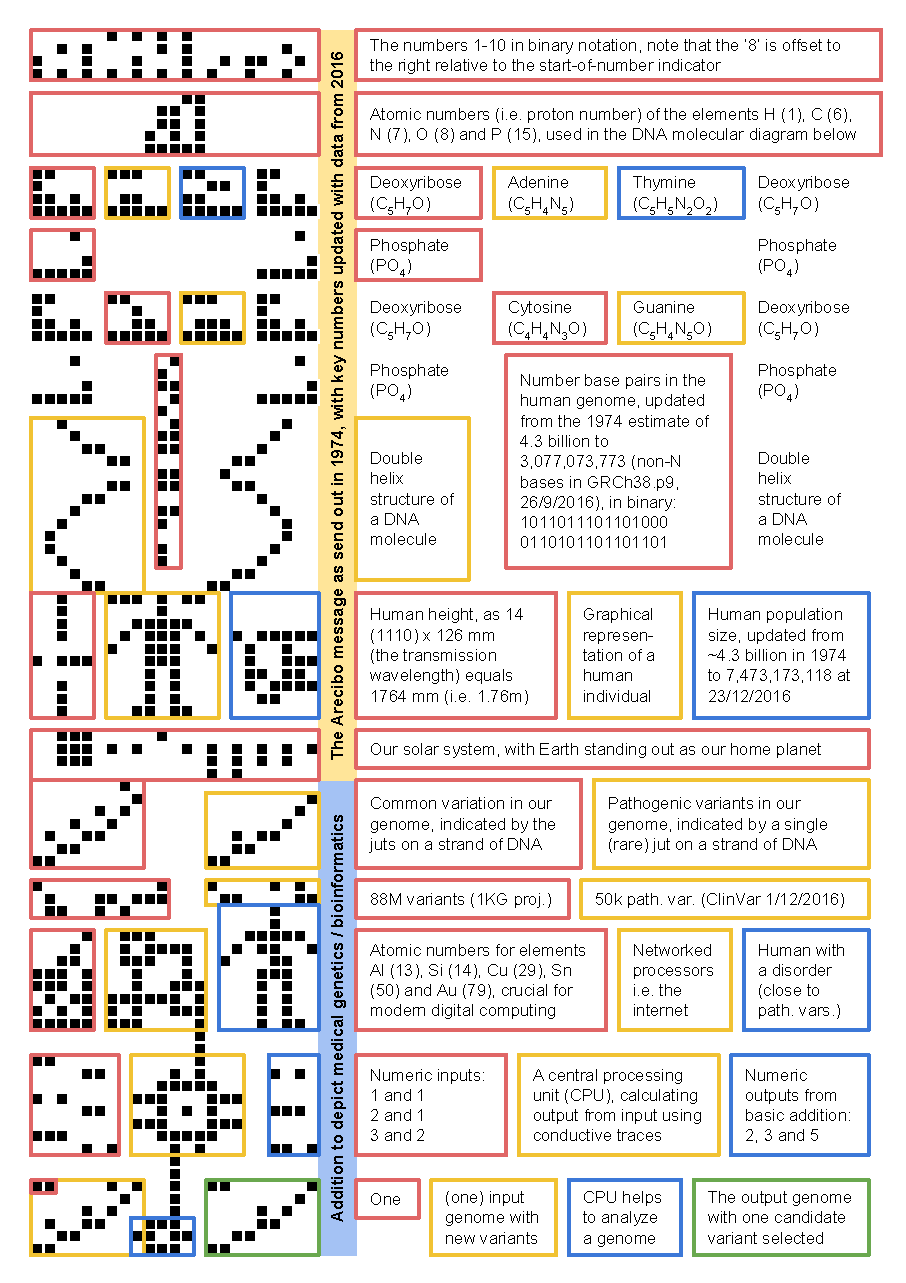
\includegraphics[scale=0.546]{img/cover_expl}